\documentclass[border=1pt]{standalone}
% inspect_style.tex: Shared style definitions for all Inspect figures
% Enforces uniform fonts, colors, and panel label positioning

\usepackage[T1]{fontenc}
\usepackage{lmodern}  % Latin Modern for Type 1 fonts
\usepackage{amssymb}  % \blacksquare for shared legends
\usepackage{pgfplots}
\usepackage{pgfplotstable}
\pgfplotsset{compat=1.18}

% Color palette (Okabe-Ito colorblind-safe, print-safe)
% -- Backbones (used wherever PatchCore vs Dinomaly are distinguished)
\definecolor{cPatchcore}{HTML}{0072B2}   % blue
\definecolor{cDinomaly}{HTML}{D55E00}    % vermillion
% -- Decision classes / gates
\definecolor{cAccept}{HTML}{009E73}      % green
\definecolor{cDefer}{HTML}{E69F00}       % orange
\definecolor{cReject}{HTML}{D55E00}      % red
\definecolor{cControl}{HTML}{56B4E9}     % light blue
\definecolor{cTransfer}{HTML}{CC79A7}    % pink
% -- Benchmarks (canonical palette; used wherever MVTec/VisA/MPDD are
%    distinguished, so benchmark colouring is uniform across all figures and
%    never collides with the backbone blue/vermillion above)
\definecolor{cMVTecAD}{HTML}{0072B2}     % blue
\definecolor{cVisA}{HTML}{E69F00}        % orange
\definecolor{cMPDD}{HTML}{009E73}        % green

% Typography defaults
\newcommand{\figfont}{\fontsize{8}{9.5}\selectfont}
\newcommand{\axislabelfont}{\fontsize{9}{10}\selectfont}
\newcommand{\titlefont}{\fontsize{9}{10}\selectfont}
\newcommand{\tickfont}{\fontsize{7}{8}\selectfont}
\newcommand{\panellabelfont}{\fontsize{9}{10}\selectfont\bfseries}

% Panel label OUTSIDE the axis (axis clip would otherwise swallow it).
% Usage after \end{axis}: \panellabel{axname}{a}
% Parked in the left gutter at the top of the axis frame — NOT on the
% title baseline — so titles can stay truly centered over the plot box.
\newcommand{\panellabel}[2]{%
  \node[anchor=south east, font=\panellabelfont, inner sep=0.5pt]
    at ([xshift=-8pt, yshift=7pt] #1.north west) {\textbf{#2}};%
}

% Standard axis styles. Titles centered above the plot box only.
\pgfplotsset{
  inspect/centertitle/.style={
    title style={at={(0.5,1.10)}, anchor=south, font=\titlefont},
  },
  inspect default/.style={
    axis x line=bottom,
    axis y line=left,
    xlabel style={font=\axislabelfont},
    ylabel style={font=\axislabelfont},
    inspect/centertitle,
    x tick label style={font=\tickfont},
    y tick label style={font=\tickfont},
    legend style={font=\tickfont, draw=none, fill=none},
  }
}


\definecolor{C_BASE}{HTML}{D55E00}
\definecolor{C_GATE}{HTML}{009E73}

% gate, baseline, row, cell, benchmark tag, deferral percent
\newcommand{\BindingRow}[6]{%
  \draw[gray!70, line width=1.1pt] (axis cs:#1,#3) -- (axis cs:#2,#3);%
  \fill[C_BASE] (axis cs:#2,#3) circle (2.2pt);%
  \fill[C_GATE] (axis cs:#1,#3) circle (2.2pt);%
  \node[anchor=east, font=\figfont, text=black] at (axis cs:-0.012,#3) {\strut\detokenize{#4} [#5]};%
  \node[anchor=west, font=\figfont, text=black] at (axis cs:0.505,#3) {#6\%};%
}

\begin{document}
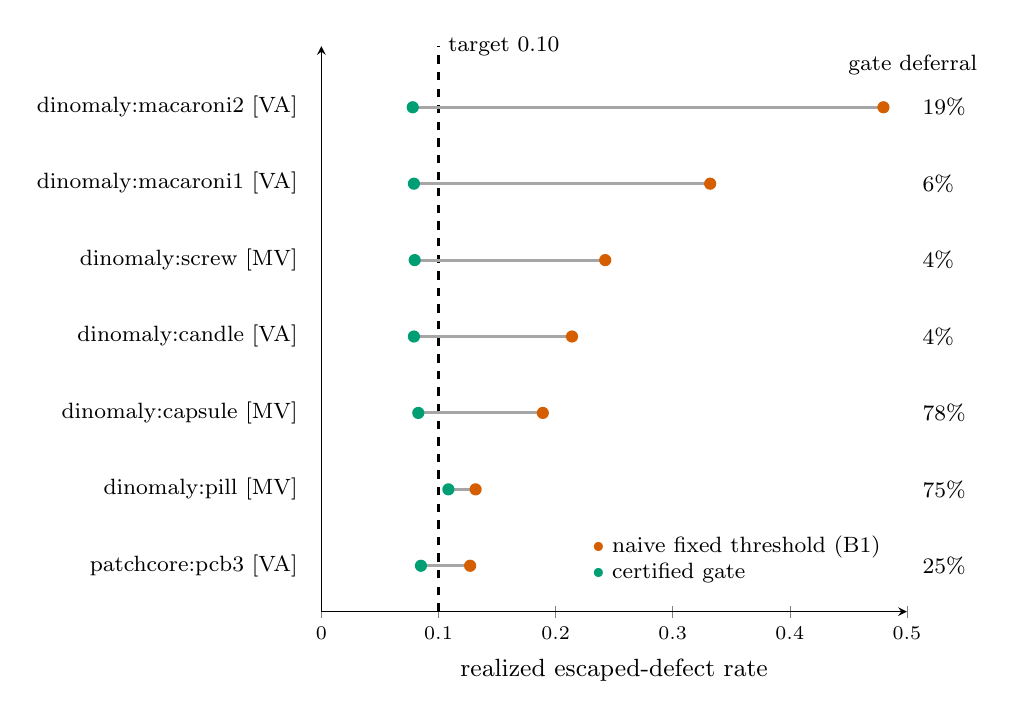
\begin{tikzpicture}[font=\figfont]
  \begin{axis}[
    inspect default,
    width=3.55in,
    height=3.45in,
    xmin=0, xmax=0.50,
    ymin=-0.6, ymax=6.8,
    xlabel={realized escaped-defect rate},
    ytick=\empty,
    axis lines*=left,
    clip=false,
  ]
    \draw[black, dashed, line width=1.0pt] (axis cs:0.10,-0.6) -- (axis cs:0.10,6.8);
    \node[anchor=south west, font=\figfont, text=black] at (axis cs:0.10,6.55) {target 0.10};

    \BindingRow{0.078}{0.48}{6}{dinomaly:macaroni2}{VA}{19}
\BindingRow{0.079}{0.3320000000000001}{5}{dinomaly:macaroni1}{VA}{6}
\BindingRow{0.07966101694915252}{0.2423728813559322}{4}{dinomaly:screw}{MV}{4}
\BindingRow{0.07900000000000001}{0.214}{3}{dinomaly:candle}{VA}{4}
\BindingRow{0.08272727272727272}{0.1890909090909091}{2}{dinomaly:capsule}{MV}{78}
\BindingRow{0.1084507042253521}{0.1316901408450704}{1}{dinomaly:pill}{MV}{75}
\BindingRow{0.08500000000000001}{0.127}{0}{patchcore:pcb3}{VA}{25}


    \node[anchor=south east, font=\figfont, text=black] at (axis cs:0.50,-0.4) {
      \begin{tabular}{l}
        \textcolor{C_BASE}{$\bullet$} naive fixed threshold (B1) \\
        \textcolor{C_GATE}{$\bullet$} certified gate
      \end{tabular}
    };
    \node[anchor=south, font=\figfont, text=black] at (axis cs:0.505,6.3) {gate deferral};
  \end{axis}
\end{tikzpicture}
\end{document}
